%!TEX root=../document.tex

\section{Ergebnisse}
\label{sec:Ergebnisse}

\subsection{Tutorial}

Zu finden ist das Tutorial entweder auf meinem Github \url{https://github.com/tfellner-tgm/SYT-rmi} \cite{repo} oder unter den Tutorials von Michael Borko \cite{bsp-command-pattern}

\subsubsection{Ant}

Ant ist ein Buildtool, welches durch die \texttt{build.xml} definiert wird.\\
Dieses File kann von eclipse oder Intellij generiert werden und besteht dann aus vielen Properties und Targets.
Die Properties bestehen als Voraussetzung f\"ur den build (z.B. Java Version, Binary Pfad ...)
Die Targets k\"onnen \"uber die Commandline ausgef\"uhrt werden mittels \texttt{ant [target]}. Der \texttt{build} target kompelliert die Sources zu Binaries, welche dann von anderen Targets verwendet werden k\"onnen. Hier k\"onnen auch Commandline-Arguments definiert werden

\subsubsection{RMI}

Konkret in dem Beispiel gibt es die Targets \texttt{engine} und \texttt{compute}, wobei Engine quasi der Server und Compute der Client ist.

Hier der wichtigste Code der Engine:

\begin{lstlisting}[style=Java, caption=Engine]
Compute engine = new ComputeEngine();
Compute stub = (Compute) UnicastRemoteObject.exportObject(engine, 0);
Registry registry = LocateRegistry.createRegistry(1099);
registry.rebind("Compute", stub);
\end{lstlisting}

Zuerst wird hier das Objekt engine erstellt. Dieses Objekt dient Compute dazu
eine Task auszuf\"uhren.
Danach wird das engine Objekt exportiert und im stub gespeichert. \\
\texttt{createRegistry(port)} erstellt eine Registry, in welcher diese stubs dann mit
dem bind oder rebind (bind w\"urde noch \"uberpr\"ufen ob der Name schon vergeben ist) mittels eines Namen freigegeben werden k\"onnen.

Die Klasse ComputePi verwendet \texttt{getRegistry(port)} um sich in die Registry
einzutragen und holt sich dann das Compute Objekt mittels \texttt{registry.lookup(name)}

\begin{lstlisting}[style=Java, caption=Compute]
Registry registry = LocateRegistry.getRegistry(1099);
Compute comp = (Compute) registry.lookup("Compute");
\end{lstlisting}

Wenn nun die Engine ausgef\"uhrt wird, bekommt man die Exception

\textcolor{red}{Java.security.AccessControlException: access denied}

\clearpage

\subsubsection{Java Policy}

RMI braucht noch bestimmte Permissions. Um dem Programm diese zu geben, muss die Datei \texttt{java.policy} unter dem Verzeichnis der JDK \texttt{/usr/lib/jvm/\{java-version\}/jre/lib/security/java.policy} ins Homeverzeichnis (\texttt{/home/\{name\}/.java.policy}) kopiert werden, wobei bei diesem Block\\

\begin{lstlisting}[caption=java.policy]
grant codeBase "file:${{java.ext.dirs}}/*" {
        permission java.security.AllPermission;
};
\end{lstlisting}

der Ausdruck \texttt{\$\{\{java.ext.dirs\}\}/*} dann noch zu \texttt{/home/\{name\}/-} ge\"andert werden muss. Dies sagt aus, dass alle Dateien (-) unter dem Homeverzeichnis diese permission haben. In diesem Fall ist alles erlaubt, wegen des Ausdrucks \texttt{java.security.AllPermission}.

\clearpage

\subsection{Command Pattern mit Callback}

\subsubsection{Command Pattern}

Das Command Pattern ist realisiert durch 2 Interfaces und deren dazugeh\"orige Klassen.

Das Command Interface gibt vor, dass ein Command die Methode \texttt{execute} besitzen muss.

\begin{lstlisting}[style=Java, caption=Command Interface]
public interface Command extends Serializable {
  	public void execute();
}
\end{lstlisting}

Das CommandExecuter Interface ist, wie der Name schon sagt, daf\"ur zust\"andig ist, die gegebenen Commands auszuf\"uhren

\begin{lstlisting}[style=Java, caption=CommandExecuter Interface]
public interface CommandExecutor extends Remote {
    public void executeCommand(Command c) throws RemoteException;
}
\end{lstlisting}

In der Konkreten Implementierung einer Klasse (\texttt{ServerService}) wird nur \texttt{c.execute()} aufgerufen.

\subsubsection{Callback}

F\"ur die Callback Funktion wurde ein Callback Interface erstellt.
Wichtig beim Interface ist, dass alle Methoden eine RemoteException werfen und die konkrete Klasse Serializable ist.

\begin{lstlisting}[style=Java, caption=Callback Interface]
public interface Callback<T> extends Remote, Serializable {
    public void set(T argument) throws RemoteException;
    public void print() throws RemoteException;
    public T receive() throws RemoteException;
}
\end{lstlisting}

\texttt{set(T argument)} dient hier als setzen eines Attributes, welches von \texttt{print()} und \texttt{receive()} verwendet wird. \\
\texttt{print()} gibt den Wert im Terminal aus.\\
\texttt{T receive()} gibt den Wert zur\"uck;

Weiters habe ich eine konkrete Klasse (\texttt{CallbackBigDecimal}) erstellt, welche diese Interface mit \texttt{BigDecimal} realisiert.

Um dann den Callback zu verwenden muss das Callback Objekt exportiert werden.
Es wird nicht in die Registry gespeichert werden, da nur der Server antworten soll und nicht irgendein anderer Client.

\begin{lstlisting}[style=Java, caption=Callback]
Callback cb = new CallbackBigDecimal();
Callback cbStub = (Callback) UnicastRemoteObject.exportObject(cb, 0);
\end{lstlisting}

\clearpage

\subsubsection{Calculation}

Das Interface Calculation wird verwendet von \texttt{PICalc} und \texttt{EulerCalc}.
Es gibt vor, dass in der Methode \texttt{calculate()} die Berechnungen gemacht werden und
in \texttt{getResult()} das Resultat zur\"uck gegeben wird.

\begin{lstlisting}[style=Java, caption=Callback Interface]
public interface Calculation {
	public void calculate();
	public BigDecimal getResult();
}
\end{lstlisting}

\texttt{PICalc} ist vom Tutorial \"ubernommen und umgeschrieben, um mit dem Interface zu funktionieren.\\
\texttt{EulerCalc} berechnet die Eulersche Zahl e mit einer bestimmten Genauigkeit.
Die Formel f\"ur die Eulersche Zahl ist \(\sum \limits_{k=0}^n e = \frac{1}{k!}\) wobei n die Genauigkeit ist.

\subsubsection{CalculationCommand}

Im \texttt{CalculationCommand} werden der Callback und die Calculation zusammengef\"uhrt.

\begin{lstlisting}[style=Java, caption=CalculationCommand Klasse]
public class CalculationCommand implements Command, Serializable {

    private static final long serialVersionUID = 12L;
    private Calculation calc;
    private Callback cb;

    public CalculationCommand(Callback cb, Calculation calc){
        this.cb = cb;
        this.calc = calc;
    }

    @Override
    public void execute() {
        System.out.println("CalculationCommand called!");
        calc.calculate();
        try {
            cb.set(calc.getResult());
            cb.print();
        } catch (RemoteException e) {
            System.out.println("Calculation Command error " + e);
        }
    }
}
\end{lstlisting}

Der Konstruktor bekommt 2 Objekte der Typen Callback und Calculation und wenn \texttt{execute()} aufgerufen wird, werden die Methoden des Interfaces aufgerufen.
Zuerst wird berechnet, dann die Nummer des Callbacks zum Resultat gesetzt und dann dieses ausgegeben.

Um das Command zu erstellen muss der vorhin erstellte callback Stub mitgegeben werden und eine neue Calculation erstellt werden\\
Hier beide M\"oglichkeiten des Programms:

\begin{lstlisting}[style=Java, caption=Command Erstellung]
Command calcPi = new CalculationCommand(cbStub, new PICalc(Integer.parseInt(args[0])));
Command calcEuler = new CalculationCommand(cbStub, new EulerCalc(args[0]));
\end{lstlisting}

\subsubsection{Programmstruktur}

Hier die Programmstruktur nochmal als ganzes in einem UML Diagramm dargestellt:\\
Die Verbindung von \texttt{Client} zu \texttt{ServerService} soll darstellen, dass das Objekt \"uber die Registry geholt wird.

\begin{figure}[!h]
        \begin{center}
                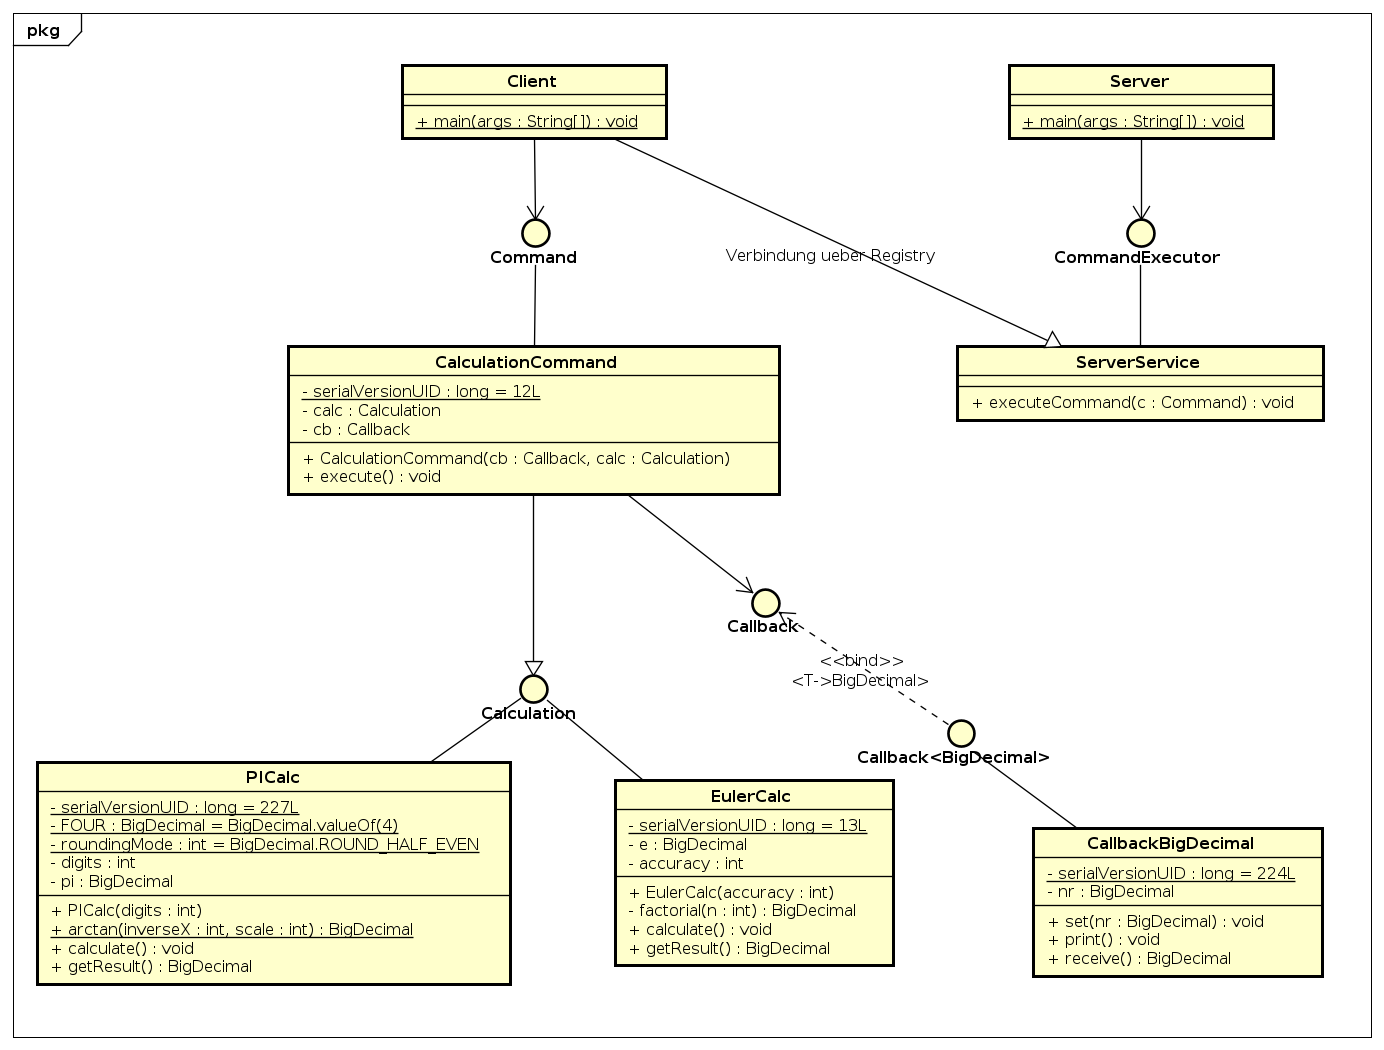
\includegraphics[width=\linewidth]{images/commandPatternUML.png}
                \caption{UML Diagramm der Aufgabe}
        \end{center}
\end{figure}

\clearpage

\section{Zeitaufzeichnung}

\renewcommand{\arraystretch}{1.5}
\begin{table}[!h]
	\center
	\begin{tabular}{ | {\hspace{3mm}} | {\hspace{3mm}} | {\hspace{3mm}} | {\hspace{3mm}} | }
		\hline \textbf{Datum} & \textbf{Erwartete Dauer} & \textbf{Reale Dauer} & \textbf{Beschreibung}\\ \hline\hline
		            22.4.2016 & 2 Stunden                & 1 1/2 Stunden        & Tutorial fertigstellen\\ \hline
                22.4.2016 & /                        & 3 1/2 Stunden        & Command Pattern und Callback \"Uberlegung \\ \hline
		            24.4.2016 & 1/2 Stunde               & 1 Stunde             & Protokoll beginnen\\ \hline
		            28.4.2016 & 2 Stunden                & 3 Stunden            & Aufgabe fertigstllen\\ \hline
		            28.4.2016 & 2 Stunden                & 3 Stunden            & Protokoll ferigstellen \\ \hline
	\end{tabular}
	\caption{Zeitaufzeichnung}
	\label{methoden}
\end{table}
